\chapter{The Fundamental Theorem of Calculus}

The Fundamental Theorem of Calculus (FTC) is a theorem that connects the
concept of differentiating a function with the concept of integrating
a function. This theorem is divided into two parts:\index{fundamental theorem of calculus}

\section{First Part}

The first part of the Fundamental Theorem of Calculus states that if
$f$ is a continuous real-valued function defined on a closed interval
$[a, b]$ and $F$ is the function defined, for all $x$ in $[a, b]$, by:

\begin{equation}
F(x) = \int_a^x f(t) \, dt
\end{equation}

Then, $F$ is uniformly continuous and differentiable on the open
interval $(a, b)$, and $F'(x) = f(x)$ for all $x$ in $(a, b)$.
(That is $F(x)$ is the antiderivative of $f(x)$.)

\section{Second Part}

The second part of the Fundamental Theorem of Calculus states that if
$f$ is a real-valued function defined on a closed interval $[a, b]$
that admits an antiderivative $F$ on $[a, b]$, and $f$ is integrable
on $[a, b]$ (it need not be continuous), then

\begin{equation}
\int_a^b f(t) \, dt = F(b) - F(a).
\end{equation}

We will also use shorthand as follows:

\begin{equation}
\int_a^b f(t)\,dt = F(t)|_a^b
\end{equation}

Which means "$F(t)$ evaluated from $t=a$ to $t=b$". 

\section{FTC and Definite Integrals}
Let $f$ be a function that is continuous on the interval $x \in \left[ a, b \right]$ and $g(x)$ is given by:
$$g(x) = \int_a^x f(t)\,dt$$
Then $g$ is continuous on $\left[a, b \right]$ and differentiable on $\left( a, b \right)$. Additionally, 
$$g'(x) = f(x)$$

\textbf{Proof}: Let $x$ and $x + h$ be in $\left( a, b \right)$. Then,
$$g(x + h) - g(x) = \int_a^{x + h} f(t)\,dt - \int_a^x f(t)\,dt$$

Recall from the chapter on definite integrals that we can split the first integral, rewriting it as:
$$g(x + h) - g(x) = \left[ \int_a^x f(t)\,dt + \int_x^{x + h} f(t)\,dt \right] - \int_a^x f(t)\,dt$$
$$g(x + h) - g(x) = \int_x^{x + h} f(t)\,dt$$

And for $h \neq 0$:
$$\frac{g(x + h) - g(x)}{h} = \frac{1}{h}\int_x^{x + h} f(t)\,dt$$

Since $f$ is continuous, there is some $u$ in $(a, b)$ such that $f(u) = m$, where $m$ is the minimum value of $f$ on the interval $(a, b)$. Similarly, there is also some $v$ such that $f(v) = M$, where $M$ is the maximum value (see figure \ref{FTCextreme}). Then we can state the true inequality that:
$$mh \leq \int_x^{x + h} f(t) \,dt \leq Mh$$
And therefore (assuming $h > 0$):
$$f(u) \leq \frac{1}{h} \int_x^{x + h} f(t)\,dt \leq f(v)$$

Substituting the equation above for the integral, we see that:
$$f(u) \leq \frac{g(x + h) - g(x)}{h} \leq f(v)$$

If we let $h$ approach zero, then the window that $u$ and $v$ are in collapses and $u$ and $v$ both approach $x$. Therefore, 
$$\lim_{h \to 0} f(u) = \lim_{u \to x} f(u) = f(x)$$

Recall also that 
$$\lim_{h \to 0} \frac{g(x + h) - g(x)}{h} = g'(x)$$

Then taking the limit as $h \to 0$ of the whole inequality becomes the Squeeze Theorem:
$$\lim_{h \to 0} f(u) \leq \lim_{h \to 0} \frac{g(x + h) - g(x)}{h} \leq \lim_{h \to 0} f(v)$$
$$f(x) \leq g'(x) \leq f(x)$$

And therefore if $g(x) = \int_a^x f(t)\,dt$, then $g'(x) = f(x)$. Notice it doesn't matter what $a$ is!

\begin{figure}[htbp]
\centering
    \begin{tikzpicture}
	\begin{axis}[xmin = 0, xmax = 6.28, axis lines = center, xlabel = $x$, x label style = {anchor = north}, xtick = {1.5, 2.094, 4.189, 5}, xticklabels = {$a$, $v$, $u$, $b$},
    ylabel = $f(x)$, y label style = {at={(axis description cs:-0.1,1.2)}, anchor = north}, ytick = {2.457, 3.826}, yticklabels = {$m$, $M$}]
        \addplot[blue, thick, domain = 0:6.28]{2*sin(deg(x)) + x};
        \draw[red, dashed](1.5, 0) -- (1.5, 6);
        \draw[red, dashed] (5, 0) -- (5, 6);
        \draw[black, dashed](2.094, 0) -- (2.094, 3.826);
        \draw[black, dashed](0, 3.826) -- (2.094, 3.826);
        \draw[black, dashed] (4.189, 0) -- (4.189, 2.457);
        \draw[black, dashed] (0, 2.457) -- (4.189, 2.457);
        \end{axis}
    \end{tikzpicture}
    \label{FTCextreme}
    \caption{$f(v) = M$, the maximum value, and $f(u) = m$, the minimum value on the interval $x \in [a, b]$}
    \end{figure}

\begin{Exercise}[label = defint5]
[This question was originally presented as a no-calculator, multiple-choice 
problem on the 2012 AP Calculus BC Exam.] Let $g$ be a continuously 
differentiable function with $g(1) = 6$ and $g'(1) = 3$. What is the value of 
$\lim_{x \to 1} \frac{\int_1^x g(t)\,dt}{g(x) - 6}$?\\
(A) 0\\
(B) $\frac{1}{2}$\\
(C) 1\\
(D) 2\\
(E) The limit does not exist\\
\vspace{40mm}
\end{Exercise}

\begin{Answer}[ref = defint5]
(D) 2. First, we try to compute the limit directly: $\lim_{x \to 1} \frac{\int_
1^x g(t)\,dt}{g(x) - 6} = \frac{\int_1^1 g(t)\,dt}{6 - 6} = \frac{0}{0}$, 
which is undefined. Because $g$ is continuous and differentiable, we can apply 
L'Hospital's rule. $\lim_{x \to 1} \frac{\int_1^x g(t)\,dt}{g(x) - 6} = \lim_{
x \to 1} \frac{d}{dx} \left[ \frac{\int_1^x g(t)\,dt}{g(x) - 6} \right] = 
\lim_{x \to 1} \frac{g(x)}{g'(x)} = \frac{g(6)}{g'(6)} = \frac{6}{3} = 2$.
\end{Answer}


\section{The Meaning of the FTC}
What the Fundamental Theorem of Calculus is really saying is that 
differentiation and integration are opposite processes. Mathematically, 
we can say $$\frac{d}{dx} \int_{a}^{x} f(t)\,dt = f(x)$$
This may seem clunky, but many useful functions are defined this way. 
Consider the Fresnel function, $S(x) = \int_{0}^{x}\sin{
\frac{\pi t^2}{2}}\,dt$. Originally used in optics, this equation is 
also used by civil engineers to design road and railway curves. 
According to FTC, then, $S'(x) = \sin{\frac{\pi t^2}{2}}$. 

We can also apply the Chain Rule when taking derivatives of integrals. 
Let $f(x) = \int_{1}^{x^4} \sec{t}\,dt$. What is $f'(x)$? First, let 
us define $u = x^4$. By the Chain Rule,
$$\frac{d}{dx}\int_{0}^{x^4} \sec{t}\,dt = \frac{d}{dx}\int_{0}^{u} 
\sec{t}\,dt$$ 
$$= \frac{d}{du}[\int_{0}^{u} \sec{t}\,dt]\frac{du}{dx}$$
$$ = \sec{u} \frac{du}{dx}$$
Noting that $\frac{du}{dx} = \frac{d}{dx}x^4 = 4x^3$, 
$$f'(x) = \sec{x^4}(4x^3)$$

\subsection{FTC Practice}
\begin{Exercise}[label=FTC1]
Use the Fundamental Theorem of Calculus to find the derivative of the 
function. 
	\begin{enumerate}
	\item $g(x) = \int_0^x \sqrt{t + t^3}\,dt$
	\item $F(x) = \int_x^0 \sqrt{1 + \sec{t}}\,dt$
	\item $h(x) = \int_1^{e^x} \ln{t}\,dt$
	\item $y = \int_{\sqrt{x}}^{\frac{\pi}{4}} \theta \tan{\theta}\,
	d\theta$
	\end{enumerate}
\end{Exercise}

\begin{Answer}[ref=FTC1]
	\begin{enumerate}
	\item $g'(x) = \sqrt{x + x^3}$
	\item $F(x) = - \int_0^x \sqrt{1+\sec{t}}\,dt$ and therefore $F'(x) = 
	- \sqrt{1+\sec{x}}$
	\item setting $u = e^x$ and noting $\frac{du}{dx} = e^x$, then $h'(x) 
	= \frac{d}{du}\int_1^{u} \ln{t}\,dt(\frac{du}{dx})$ Taking the 
	derivative and substituting for $\frac{du}{dx}$, we find $h'(x) = 
	\ln{u} \cdot e^x = \ln{(e^x)} \cdot e^x = x \cdot e^x$
	\item $y = - \int_{\frac{\pi}{4}}^{\sqrt{x}} \theta \tan{\theta}\,
	d\theta$. Setting $u = \sqrt{x}$ and noting that $\frac{du}{dx} = 
	\frac{1}{2\sqrt{x}}$, we see that $y' = -\frac{d}{du}
	[\int_{\frac{\pi}{4}}^{u}\theta\tan{\theta}\,d\theta]\frac{du}{dx} 
	= u\tan{u} \cdot \frac{1}{2\sqrt{x}} = -\sqrt{x}\tan{\sqrt{x}} \cdot 
	\frac{1}{2\sqrt{x}} = \frac{-\sqrt{x}\tan{\sqrt{x}}}{2\sqrt{x}} = 
	- \frac{1}{2}\tan{\sqrt{x}}$
	\end{enumerate}
\end{Answer}

\section{Using Antiderivatives to Evaluate Definite Integrals}
In everyday English, the FTC states that the integral from $a$ to $b$ 
of a function is the antiderivative of that function evaluated from 
$a$ to $b$. In the previous chapter, the integrals presented were of 
linear functions where the area under the curve could be equally 
calculated by hand. The FTC connects integrals to antiderivatives, 
allowing us to evaluate more complex integrals. Consider the following 
example:\\

The power consumption of a household can be modeled as 
$P(t) = \frac{1}{10} t^2 (t - 24)^2$ from $t = 0$ to $t = 24$, where 
$P$ is measured in watts and $t$ is measured in hours ($t = 0$ is 
midnight). The total energy the household uses is given by $\int_{0}^{24} 
P(t)\,dt$. As you can see from the graph (see figure \ref{fig:power}), 
we cannot simply use our geometry skills to determine the area under 
the curve. 

\begin{figure}
	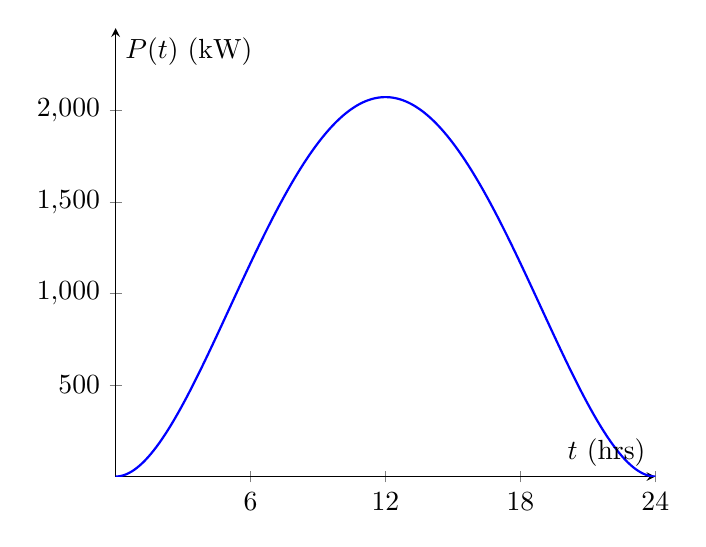
\begin{tikzpicture}
		\begin{axis}
		[axis lines = center, xmin = 0, xmax = 24, xlabel = $t$ (hrs),
		ymin = 0, ymax = 2450, ylabel = $P(t)$ (kW),
            xtick={6, 12, 18, 24}]
		\addplot[blue, thick, samples=200, domain =0:24] {0.1*x^2*(x-24)^2};
		\end{axis}
	\end{tikzpicture}
	\caption{Power consumption of a household in a day}
	\label{fig:power}
\end{figure}

To determine the total energy use, we need to evaluate $\int_{0}^{24} 
\frac{1}{10}t^2(t-24)^2\,dt$. First, we expand the polynomial:\\
$$E_{tot} = \frac{1}{10} \int_{0}^{24} t^2 (t^2-48t+576)\,dt = 
\frac{1}{10}\int_{0}^{24} t^4 - 48t^3 + 576t^2\,dt$$
$$= \frac{1}{10}\int_{0}^{24} t^4\,dt - \frac{24}{5}\int_{0}^{24} 
t^3\,dt + \frac{288}{5}\int_{0}^{24} t^2\,dt$$\\
Using the Power Rule to determine the antiderivatives of $t^4$, $t^3$, 
and $t^2$, we see:\\
$$=\frac{1}{10}[\frac{1}{5}t^5]|_{0}^{24} - \frac{24}{5}
[\frac{1}{4}t^4]|_{0}^{24} + \frac{288}{5}[\frac{1}{3}t^3]|_{0}^{24} 
= 26542.1 Whr = 26.5421 kWhr$$

\subsection{Definite Integrals Practice}
\begin{Exercise}[label=FTC2]
	Evaluate the following integrals:
	\begin{enumerate}
	\item $\int_1^4 t^{-3/2}\,dt$
	\end{enumerate}
\end{Exercise}

\begin{Answer}[ref=FTC2]
	\begin{enumerate}
	\item The antiderivative of $t^{-3/2}$ is $\frac{-2}{\sqrt{t}}$. 
	Therefore, the integral is equal to $[\frac{-2}{\sqrt{t}}]_1^4 = 
	\frac{-2}{\sqrt{4}} - \frac{-2}{\sqrt{1}} = -1 + 2 = 1$. 
	\end{enumerate}
\end{Answer}

\begin{Exercise}[label=FTC3]
	[This question was originally presented as a multiple-choice, 
	no-calculator problem on the 2012 Calculus BC exam.] The graph of a 
	differentiable function $f$ is shown in the graph. $h(x) = \int_0^x 
	f(t)\,dt$. Rank the relative values of $h(6)$, $h'(6)$, and $h''(6)$ 
	from lowest to highest.
	
	\begin{tikzpicture}
		\begin{axis}
		[axis lines = center, xlabel = $x$, ylabel = $f(x)$,
		xmin = 0, xmax = 9, xtick = {1, 2, 3, 4, 5, 6, 7, 8, 9},
		ymin = -4, ymax = 2, ytick = {-4, -3, -2, -1, 1, 2}]
		\addplot[blue, thick, samples=100, domain = 0:9]
		{2.5*sin(30*(x+6.6))-0.75};
		\end{axis}
	\end{tikzpicture}
\end{Exercise}

\begin{Answer}[ref=FTC3]
According to FTC, $h'(x) = f(x)$ and $h''(x) = f'(x)$. Examining the 
graph, we see that the curve lies below the $x$-axis for $0<x<6$, 
which means that $h(6) = \int_0^6 f(t)\,dt < 0$. $h'(6) = f(6) = 0$ 
and $h''(6) = f'(6) > 0$. Therefore, $h(6) < h'(6) < h''(6)$. 
\end{Answer}

\begin{Exercise}[label=defint6]
	The graph of $f'$ is shown in the graph and consists of a semi-circle 
	and two line segments. If $f(2) = 1$, then what is $f(-5)$?\\
	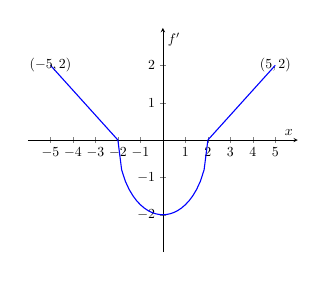
\begin{tikzpicture}[scale = 0.5]
		\begin{axis}
		[axis lines = center, xmin = -6, xmax = 6, xlabel = $x$,
		xtick = {-5, -4, -3, -2, -1, 1, 2, 3, 4, 5},
		ymin = -3, ymax = 3, ylabel = $f'$, ytick = {-2, -1, 2, 1}]
		\addplot[blue, thick]coordinates{(-5, 2) (-2, 0)};
		\node[] at (5, 2) {$(5, 2)$};
		\node[] at (-5, 2) {$(-5, 2)$};
		\addplot[blue, thick]coordinates{(5, 2) (2, 0)};
		\addplot[blue, thick, domain = -2:2]{- sqrt(4 - x^2)};
		\end{axis}
	\end{tikzpicture}
\end{Exercise}

\begin{Answer}[ref=defint6]
	We know that $f(2) = \int_{-5}^2 f'(x)\,dx + f(-5)$. Examining the 
	graph, we know that $\int_{-5}^2 f'(x)\,dx = frac{1}{2}(3)(2) - 
	\frac{1}{2}\pi(2^2)$ (the area of the triangle above the $x$-axis 
	less the area of the semi-circle below the axis). Therefore, $f(-5) 
	= f(2) - \int_{-5}^2 f'(x)\,dx = 1-(3-2\pi) = 2\pi-2$
\end{Answer}

\begin{Exercise}[label = defint7]
[This question was originally presented as a calculator-allowed, multiple-
choice question on the 2012 AP Calculus BC exam.] A particle moves along a 
line so that its acceleration for $t \geq 0$ is given by $a(t) = \frac{t + 3}{
\sqrt{t^3 + 1}}$. If the particle's velocity at $t = 0$ is $5$, what is the 
velocity of the particle at $t = 3$?
\end{Exercise}

\begin{Answer}[ref = defint7]
11.71. The particle's velocity will be given by its initial velocity plus the 
integral of its acceleration over the time period. Therefore, $v(3) = v(0) + 
\int_0^3 a(t)\,dt = 5 + \int_0^3 \frac{t + 3}{\sqrt{t^3 + 1}}\,dt \approx 5 + 
6.71 = 11.71$. 
\end{Answer}

\section{Average Value of a Function}
The average value of a function, $f$, on an interval $\left[ a, b \right]$ is 
given by:
\begin{mdframed}[style=important, frametitle={Average Value of a Function}]
$$f_{avg} = \frac{1}{b - a} \int_a^b f(x)\,dx$$
\end{mdframed}

\textbf{Example}: Find the average value of $f(x) = 3 + x^2$ on the interval 
$[-2, 1]$. 

\textbf{Solution}: Taking $a = -2$ and $b = 1$, we have:
$$f_{avg} = \frac{1}{1 - (-2)} \int_{-2}^1 \left[ 3 + x^2 \right]\,dx$$
$$f_{avg} = \frac{1}{3} \int_{-2}^1 \left[ 3 + x^2 \right]\,dx$$
$$f_{avg} = \frac{1}{3} \left[3x + \frac{1}{3}x^3 \right]_{x = -2}^{x = 1}$$
$$f_{avg} = \frac{1}{3} \left[ \left( 3 \cdot 1 + \frac{1}{3} \cdot 1^3 \right) 
- \left( 3 \cdot (-2) + \frac{1}{3} \cdot (-2)^3 \right) \right]$$
$$f_{avg} = \frac{1}{3} \left[ \left(3 + \frac{1}{3} \right) - \left(-6 - 
\frac{8}{3} \right) \right]$$
$$f_{avg} = \frac{1}{3} \left[ \frac{10}{3} + 6 + \frac{8}{3} \right] = 
\frac{1}{3}(12) = 4$$

Therefore, the average value of $f(x) = 3 + x^2$ on the interval $\left[ -2, 1 
\right]$ is 4. 

\begin{Exercise}[label = func_avg]
[This question was originally presented as a multiple-choice, calculator-
allowed problem on the 2012 AP Calculus BC Exam.] What is the average value of 
$y = \sqrt{\cos{x}}$ on the interval $0 \leq x \leq \frac{\pi}{2}$?
\end{Exercise}

\begin{Answer}[ref = func_avg]
We begin by setting up the integral for average value of a function with $a = 
0$, $b = \frac{\pi}{2}$, and $f(x) = \sqrt{\cos{x}}$:
$$\frac{1}{\pi / 2 - 0} \int_0^{\pi / 2} \sqrt{\cos{x}}\,dx$$
$$= \frac{2}{\pi} \int_0^{\pi/2} \sqrt{\cos{x}}\,dx$$
There's not an obvious way to evaluate this integral by hand. Luckily, this 
question allows for the use of a calculator. Entering this integral into a 
calculator (such as a TI-89 or Wolfram Alpha), we find that:
$$\frac{2}{\pi} \int_0^{\pi/2} \sqrt{\cos{x}}\,dx \approx 0.763 $$
\end{Answer}